\documentclass{article}
\usepackage[a4paper,bindingoffset=0.2in,%
            left=0.5in,right=1in,top=1in,bottom=1in,%
            footskip=.25in]{geometry}
\usepackage{minted}
\usepackage{graphicx} %TO include graphics in document
\begin{document}
\title{Python Programs for `DDoS Detection and Mitigation Using Machine Learning Tools'}
\author{Arpit Gawande}
\maketitle
\newpage
\section{Data extraction from Wireshark capture file}

\textbf{\large{Library imports}}
\begin{minted}{Python}
#Pandas for creating data-frames
import pandas as pd

#Pyshark to capture packets
import pyshark
#For file operarions
import os
import gc
import sys
\end{minted}
\textbf{\large{Define required attributed needed to extract from capture.}}
\begin{minted}{Python}
required_keys = ['ip.dst', 'ip.proto', 'tcp.flags.syn', 'tcp.flags.ack']
\end{minted}
\textbf{\large{Reading packets from pre-captured file using Pyshark}}
\begin{minted}{Python}
file_cap = pyshark.FileCapture('captures/botnet-capture-20110810-neris.pcap')
\end{minted}
\textbf{\large{Extract IP packets from the captured file for further processing}}
\begin{minted}{Python}
%time
#Write extraction result to
base_directory = 'converted/test3/attack_samples/1/'
#Debugger for pyshark
#file_cap.set_debug()
#Attributes for sample size
startTime = 0.0
endTime = 0.0
i = -1
first = True
#Sample Number
init_sample = 1
dfList = []
while(True):
    i += 1
    #Each packet can have multiple layers (e.g eth, ip, tcp etc.).
    #Combine them in list for a single packet.
    layerList = []
    #pyshark not able to handle AttributeError, AssertionError and KeyError(index values)
    try:
        #Iterate through layer of packet
        for layer in file_cap[i]:
            # Slice Data according to time
            t = float(file_cap[i].sniff_timestamp)
            #Initial setup
            if startTime == 0.0:
                startTime = t
                endTime = startTime + 300 # 300 sec(5 min) is the sample size
                sample = init_sample
                print(sample, startTime, endTime)
            # Write every sample to csv file
            elif t > endTime:
                if not os.path.exists(base_directory):
                    os.makedirs(base_directory)
                dfList.to_csv(base_directory+str(sample))
                #Clear list after writing this would save memory
                startTime = endTime
                endTime = startTime + 300
                sample += 1
                #Reset after writing to file
                first = True
                print(sample, startTime, endTime)
                gc.collect()
            #We need only ip layer only
            if layer._layer_name == 'ip':
                #Layer values are in the form of dictionary. Filter the attributes
                layer_dict = {key:value for key, value in layer._all_fields.items()
                              if key in required_keys}
                #Create data-frame from dictionary
                layerList.append(pd.DataFrame(layer_dict, index=[0]))
                #Add timestamp and sample number
                layerList.append(pd.DataFrame({'sniff_timestamp':file_cap[i].sniff_timestamp},
                                              index=[0]))
                layerList.append(pd.DataFrame({'sample':sample}, index=[0]))
                #Build packet dataframe from layer frames. Its single row dataframe
                cDf = pd.concat(layerList, axis=1);
                if first:
                    dfList = cDf
                    first = False
                else:
                    dfList = dfList.append(cDf, ignore_index=True)
    except (AttributeError, AssertionError) as e:
        continue  #print('Ipv4 packet does not exist')
    except  KeyError:
        break;

#If sample data is not written to file because for frame size
if(sample == init_sample):
    dfList.to_csv(base_directory+str(init_sample))
\end{minted}

\pagebreak
\section{DDoS attack Detection based on destination IP address}

\textbf{\large{Library imports}}
\begin{minted}{Python}
#Pandas for creating data-frames
import pandas as pd

#Pyshark to capture packets
import pyshark
#For file operations
import os
import gc
import sys
\end{minted}
\textbf{\large{Declare and define file/folders for storing/retrieving data for analysis}}
\begin{minted}{Python}
#Base Folder Paths
base_folder_name = 'converted'
test_folder_name = 'test2'
base_path = os.path.join(base_folder_name, test_folder_name)
#Normal Sample and cluster paths
sample_dir_name = 'samp'
sample_path = os.path.join(base_path, sample_dir_name)
#If sample folder exist
if os.path.isdir(sample_path):
    #Test and Train data Folders
    sample_train_path = os.path.join(base_path, sample_dir_name+'_train')
    os.makedirs(sample_train_path, exist_ok=True)
    sample_test_path = os.path.join(base_path, sample_dir_name+'_test')
    os.makedirs(sample_test_path, exist_ok=True)
    #Clustering folders
    cluster_train_path = os.path.join(sample_train_path, 'cluster')
    os.makedirs(cluster_train_path, exist_ok=True)
    cluster_test_path = os.path.join(sample_test_path, 'cluster')
    os.makedirs(cluster_test_path, exist_ok=True)
\end{minted}
\textbf{\large{Defining features we want to work with}}
\begin{minted}{Python}
features = [1, 6, 17] #(ICMP:1, TCP:6, UDP:17)
\end{minted}
\textbf{\large{Creating feature tables which would be input to k-means learning algorithms}}
\begin{minted}{Python}
def get_feature_dataframe(sample_file, features):
    """
    Create feature table from the sample file which has flow information

    Parameters
    ----------

    sample_file: string
        file(full path) containing IP layer information destination address,
        protocol, time stamp.

    features: list
        list of feature we required for anlysis.
    """
    df = pd.read_csv(sample_file, index_col=0)
    #Filter Columns
    df = df[['ip.dst', 'ip.proto', 'sniff_timestamp', 'sample']]
    #Remove null destinations
    df = df[df['ip.dst'].notnull()]
    #Rename Columns
    df.columns = ['ip', 'protocol', 'time_stamp', 'sample']
    #Get count for each ip
    df = df.groupby(['ip', 'protocol']).size().unstack().fillna(0).astype(int)
    #Drop row for given IP
    #df = filter_ip(df, '147.32.84.165')
    if(set(df.columns) != set(features)):
        non_columns = set(features) - set(df.columns)
        for c in non_columns:
            df.insert(loc=features.index(c), column=c, value=0)
    #Select only required protocols which would be used as features
    df = df[features]
    return df
\end{minted}
\begin{minted}{Python}
#Merge sample files to create bigger samples
def merge_files(files, merge_count, features):
    """
    Merge feature sample file to form bigger sample.

    Parameters
    ----------
    files: list
        all the sample files,

    merge_count: int
        number of files to be merged.

    features: list
        list of features

    """
    if len(files) < merge_count:
        print('Too few file to merge')
        return
    dfs = []
    count = 0
    for file in files:
        if count == 0:
            df = get_feature_dataframe(file, features)
            count += 1
        else:
            temp_df = get_feature_dataframe(file, features)
            df = df.append(temp_df)
            count += 1
        if count == merge_count:
            df = df.groupby(df.index).sum()
            dfs.append(df)
            count = 0
    return dfs
\end{minted}
\begin{minted}{Python}
def create_train_test(sample_path, features, merge_count=1):
    """
    Seperate data into train and test for the evaluation of the algorithms

    Parameters
    ----------

    sample_path: string
        location where all the packet sample files are kept

    merge_count: int, default 1
        Number of files to be merged to create a feature table

    feature: list
        List of features to be considered for creating feature table
    """
    files = sorted(glob.glob(os.path.join(sample_path,'*')),  key=os.path.getmtime)

    test_files = files[:merge_count]
    train_files = files[merge_count:]

    test_dfs = merge_files(test_files, merge_count, features)
    train_dfs = merge_files(train_files, merge_count, features)

    return train_dfs, test_dfs, merge_count
\end{minted}
\textbf{Create train and test data frames}
\begin{minted}{Python}
train_dfs, test_dfs, merge_count = create_train_test(sample_path, features)
\end{minted}
\textbf{Save merge count which will be used for merging the files to form larger sample.}
\begin{minted}{Python}
np.savetxt(os.path.join(base_path, 'merge_count'),
           np.asarray(merge_count).reshape(1,), fmt='%d')
\end{minted}
\textbf{Store train and test tables on the file system}
\begin{minted}{Python}
#Write train and test data to file
train_files = []
for i, df in enumerate(train_dfs, 1):
    train_file = os.path.join(sample_train_path,str(i))
    df.to_csv(train_file)
    train_files.append(train_file)
test_files = []
for i, df in enumerate(test_dfs, 1):
    test_file = os.path.join(sample_test_path,str(i))
    df.to_csv(test_file)
    test_files.append(test_file)
\end{minted}
\pagebreak
\section{k-means clustering}
\textbf{\large{Functions for finding optimal number of clusters for k-means clustering algorithm using elbow method.}}
\begin{minted}{Python}
#Find optimal number of clusters for k-means clustering using elbow method.
def elbow_method(X_trans, ax, title):
    """
    For the k-means algorithm, elbow method check the percent of
    variance explained as function of the number of clusters.
    Variance for each cluster number is calculated and the cluster
    number which produce less variance for the next cluster number
    is selected as best choice.

    Parameters
    ----------

    X_tran: vector
        Standardize vector.
    """
    elbow_count = 0
    range_val = 10
    nc = range(1, range_val)
    kmeans = [KMeans(n_clusters=i) for i in nc]
    score = [kmeans[i].fit(X_trans).score(X_trans) for i in range(len(kmeans))]
    total_diff = abs(score[0] - score[len(score) -1])
    for i in range(range_val - 2):
        percent_diff = abs(score[i] - score[i+1])/total_diff
        if percent_diff < 0.01:
            opt_clust_count = i
            break
    ax.plot(nc,score)
    ax.set_xlabel('Number of Clusters')
    ax.set_ylabel('Score')
    ax.set_title(title)
    return opt_clust_count
\end{minted}
\begin{minted}{Python}
def get_optimal_cluster_count(df_list, count):
    """
    Apply elbow method on all the sample vectors and get their mean as
    the best cluster number for kmeans algorithm.

    Parameters
    ----------

    df_list: list of dataframes
        contain tables/dataframes for each sample data.

    count: int
        Number of sample to loop t.
    """
    elbow_vals = []
    row_count = math.ceil(count/2)
    fig = plt.figure(figsize=(10, 4*row_count), dpi=80, facecolor='w', edgecolor='k')
    fig.subplots_adjust(hspace=.5) #Adjust space between the subplot
    for i, df in enumerate(df_list[:count], 1):
        X = df.values
        #Create scaling and transforme
        X_trans = preprocessing.StandardScaler().fit_transform(X)
        #Create subplot
        ax = fig.add_subplot(row_count, 2, i)
        title = 'Sample:'+str(i)
        fig.suptitle('Elbow Method', fontsize=16)
        elbow = elbow_method(X_trans, ax, title)
        elbow_vals.append(elbow)
    plt.savefig('elbow-method.png')
    return int(np.floor(np.mean(elbow_vals)))
\end{minted}
\textbf{Get the optimal cluster count}
\begin{minted}{Python}
sample_count = 4 #Number of samples to be used for elbow method
cluster_count = get_optimal_cluster_count(train_dfs, sample_count)
\end{minted}

\begin{figure}[H]
\centering
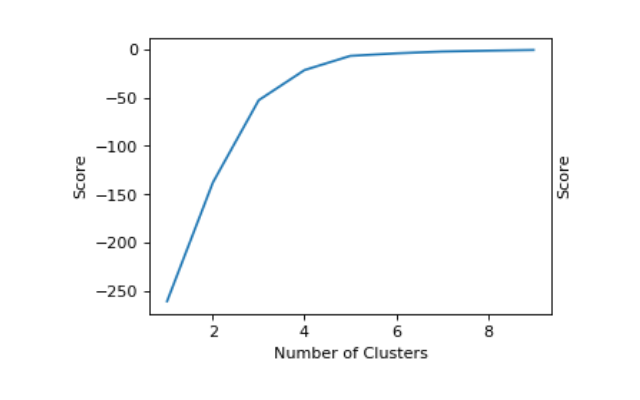
\includegraphics[width=0.90\textwidth]{elbow-method.png}
\caption{Elbow Method for cluster count detection} \label{fig:elbow-method-in-program}
\end{figure}

\pagebreak
\textbf{\large{Functions for finding and storing the centroid which would be used for all k-means clustering.}}
\begin{minted}{Python}
def get_kmeans_centroid(feature_df, cluster_count):
    """
    Run the k-means algorithm on input data vector and find out the
    centroid for each cluster then return that centroid in the
    form of table

    Parameters
    ----------

    feature_df: table/dataframe
        vector on which the k-means algorithm is be applied

    cluster_count: int
        Number of clusters to be used for k-means clustering
    """
    df_centroid = {}
    X = feature_df.values
    #Create scaling
    scaler = preprocessing.StandardScaler().fit(X)
    #Transform Training data
    X_trans = scaler.transform(X)
    #Data Fitting using K-means
    kmeans = KMeans(n_clusters=cluster_count)
    kmeans.fit(X_trans)
    #Create cluster data-frame for saving on file system
    #Dataframe 0 contain all the clusters centers associated with 0th cluster
    first = True
    for i in range(kmeans.cluster_centers_.shape[0]):
        s = pd.Series(kmeans.cluster_centers_[i], index=feature_df.columns)
        if(first):
            df_centroid = pd.DataFrame(columns=feature_df.columns)
            first = False
        df_centroid = df_centroid.append(s,ignore_index=True)
    return df_centroid
\end{minted}
\begin{minted}{Python}
def get_kmeans_cluster_centroids(sample_frames, features, cluster_count):
    """
    This function will first find all cluster centroids for all the
    training sample vectors and then calculate the median of each
    cluster over all the samples. This median would be the best guess
    of the centroid for all the training vectors and also would be use
    for evaluation.

    Parameters
    ----------

    sample_frames: list
        list of feature vector datafames.

    features: list
        list of feature.

    cluster_count: int
        number of clusters to be considered for k-means clustering.

    """
    df_concat = pd.DataFrame(columns=features)
    for df in sample_frames:
        #Run kmeans and get centroid
        df_centroid = get_kmeans_centroid(df, cluster_count)
        #Create list of centroids
        df_concat = df_concat.append(df_centroid)
    centroids = []
    #Find median for each centroid and store them in file
    for c in range(cluster_count):
        med = np.median(df_concat.loc[c], axis=0) # e.g. df_concat.loc[0] is df of clister 0
        centroids.append(med)
    return centroids
\end{minted}
\textbf{Find the median of all the centroids. This median is the better estimation of the centroids for
all future k-means clustering. Store it on the file system. Also store the feature list on file system:}
\begin{minted}{Python}
#Already define base directory path
base_path = base_path
#File to store centroids
centroid_filename = 'centroids.csv'
#File to store feature list
features_filename = 'features.csv'

#Call to find median of centroid
centroids = get_kmeans_cluster_centroids(train_dfs, features, cluster_count)

#Save centroids and features in files for future use
np.savetxt(os.path.join(base_path, centroid_filename),
           np.asarray(centroids), delimiter=",")
np.savetxt(os.path.join(base_path, features_filename),
           np.asarray(list(features)), delimiter=",")
\end{minted}
\begin{minted}{Python}
def read_centroid_features(base_path, centroid_filename, features_filename):
    """
    Read previously calculated centroids and stored feature from the file system.

    Parameters
    ----------

    base_path: string
        folder location in which both centroids and feature file are present

    centroid_filename: string
        Name of the file in which centroid vector is stored.

    features_filename: string
        Name of the file in which feature list is stored.

    """
    centroids = np.genfromtxt(os.path.join(base_path,centroid_filename), delimiter=',')
    features = np.genfromtxt(os.path.join(base_path,features_filename), delimiter=',')
    features = list(features.astype('int64'))
    return centroids, features
\end{minted}
\textbf{\large{After finding cluster count and the common centroids we will be doing kmeans
clustering using previously calculated centroids}}
\begin{minted}{Python}
#Base directory path
base_path = base_path #Already define
#File to store centroids
centroid_filename = centroid_filename #Already define
#File to store feature list
features_filename = features_filename #Already define
#Get centroids and feature
centroids, features = read_centroid_features(base_path,
                                             centroid_filename, features_filename)
\end{minted}
\textbf{\large{Plot k-means clustering for samples}}
\begin{minted}{Python}
def draw_clusters(X, pre_centroids, ax, title):
    """
    Draw clusters in 2D

    Parameters
    ----------

    X: vector
        vector to be clustered and plot.

    ax: object
        pyplot subplot object for plotting the clusters.

    title: string
        title of the plot.

    """
    if X.shape[1] > 2:
        #Use PCA component analysis for 2D visuals
        reduced_X = PCA(n_components=2).fit_transform(X)
        km = KMeans(n_clusters=pre_centroids.shape[0])
        km.fit(reduced_X)
    else:
        reduced_X = X
        km = KMeans(n_clusters=pre_centroids.shape[0], init=pre_centroids)
        km.fit(reduced_X)

    # Step size of the mesh. Decrease to increase the quality of the VQ.
    h = .01     # point in the mesh [x_min, x_max]x[y_min, y_max].

    # Plot the decision boundary. For that, we will assign a color to each
    x_min, x_max = reduced_X[:, 0].min() - 1, reduced_X[:, 0].max() + 1
    y_min, y_max = reduced_X[:, 1].min() - 1, reduced_X[:, 1].max() + 1
    xx, yy = np.meshgrid(np.arange(x_min, x_max, h), np.arange(y_min, y_max, h))

    # Obtain labels for each point in mesh. Use last trained model.
    Z = km.predict(np.c_[xx.ravel(), yy.ravel()])

    # Put the result into a color plot
    Z = Z.reshape(xx.shape)
    plt.imshow(Z, interpolation='nearest',
               extent=(xx.min(), xx.max(), yy.min(), yy.max()),
               cmap=plt.cm.Paired,
               aspect='auto', origin='lower')

    #Plot the data points
    ax.plot(reduced_X[:,0],reduced_X[:,1],  'k.', markersize=3)
    # Plot the centroids as a white X
    centroids = km.cluster_centers_
    ax.scatter(centroids[:, 0], centroids[:, 1], marker='x', s=169,
               linewidths=3, color='w', zorder=10)
    #Set tile and boundaries of the plot
    ax.set_title(title)
    ax.set_xlim(x_min, x_max)
    ax.set_ylim(y_min, y_max)
    ax.set_xticks(())
    ax.set_yticks(())
\end{minted}
\begin{minted}{Python}
def plot_kmeans_clusters(to_print_df):
    fig = plt.figure(figsize=(10, 8), dpi=80, facecolor='w', edgecolor='k')
    row_count = math.ceil(len(to_print_df)/2)
    for i, df in enumerate(to_print_df, 1):
        X = df.values
        #Create scaling
        X_trans = preprocessing.StandardScaler().fit_transform(X)
        #Create subplot
        ax = fig.add_subplot(row_count, 2, i)
        plt.suptitle('k-means++ clustering (with PCA-reduced data)', fontsize=16)
        title = 'Sample:'+str(i)
        draw_clusters(X_trans, centroids, ax, title)
    plt.savefig('kemans-clustering.png')
\end{minted}
\textbf{Plot only few clusters as not all required.}
\begin{minted}{Python}
plot_count = 4
to_print_df = train_dfs[:plot_count]
plot_kmeans_clusters(to_print_df)
\end{minted}

\begin{figure}[H]
\centering
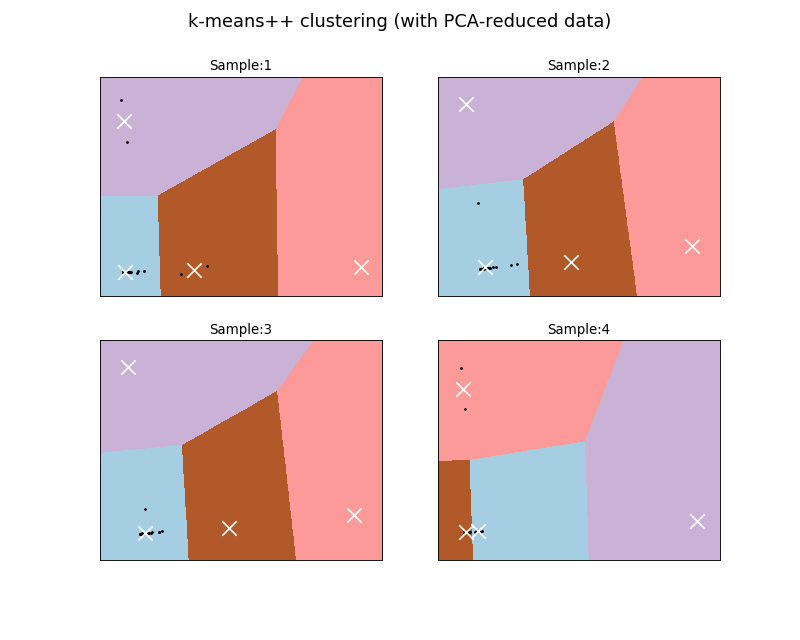
\includegraphics[width=0.90\textwidth]{kemans-clustering.png}
\caption{Clustering using k-means++ algorithm} \label{fig:kmeans-clustering-in-program}
\end{figure}
\pagebreak
\textbf{\large{Do k-means++ clustering and save clustered output in the files}}
\begin{minted}{Python}
def kmeans_clustering(feature_df, centroids):
    """
    Clustering input vector using k-means algorithm

    Parameter
    ---------
    feature_df: Object
        Panda dataframe object containing input vector which
        is to clustered using k-means.

    centroids: vector
        Vector containing centroid values. These centroids are
        used for clutering.

    """
    X = feature_df.values
    #Create scaling
    scaler = preprocessing.StandardScaler().fit(X)
    #Transform Training data
    X_trans = scaler.transform(X)
    #k means clustering using provided centroids
    kmeans = KMeans(n_clusters=centroids.shape[0], init=centroids)
    clusters = kmeans.fit_predict(X_trans)
    #Getting the labels/clusters for each IP
    cluster_df = pd.DataFrame({'cluster': kmeans.labels_})
    #Attaching labels to existing dataframe and return new dataframe
    df = pd.concat([feature_df.reset_index(), cluster_df], axis=1).set_index('ip')
    return df
\end{minted}
\textbf{\large{Apply clustering on both training and test data. Store clustered information on the file system}}
\begin{minted}{Python}
#First retrieve the centroids and features
centroids, features = read_centroid_features(centroid_filename, features_filename)
\end{minted}
\textbf{Cluster all the samples and store them on file.}
\begin{minted}{Python}
centroids, features = read_centroid_features(centroid_filename, features_filename)
for i, train_df in enumerate(train_dfs):
    clustered_df = kmeans_clustering(train_df, centroids)
    clustered_df.to_csv(os.path.join(cluster_train_path,str(i+1)))
for i, test_df in enumerate(test_dfs):
    clustered_df = kmeans_clustering(test_df, centroids)
    clustered_df.to_csv(os.path.join(cluster_test_path,str(i+1)))
\end{minted}
\textbf{\large{Now combine clustering of all the train/test samples and find out the best cluster and average packet count for each IP}}
\begin{minted}{Python}
def get_best_cluster_sample_count(cluster_path):
    """
    Get all the trained IP address and then combine training data
    from all the sample to make best judgment about the cluster
    in which IP address should be placed into. It also gives the
    average number of packets flowing during the analysis time
    which would help to determine if its truly attack or
    just a misjudgment.

    Parameters
    ----------

    cluster_path: string
        directory location where the clustered samples are stored.

    """
    files = sorted(glob.glob(os.path.join(cluster_path,'*')),  key=os.path.getmtime)
    first = True
    for file in files:
        if first:
            df = pd.read_csv(file, index_col=0)
            first = False
        else:
            temp_df = pd.read_csv(file, index_col=0)
            df = df.append(temp_df)
    #Fist reindex all data with IP
    df = df.reset_index().set_index(['ip'])

    new_columns =  ['cluster', 'packet_count']
    features = list(df.columns[:-1])
    cluster_column = list(df.columns[-1:])
    #Average packet count across all the samples
    packet_count = df[features].groupby('ip').mean().sum(axis=1).astype('int64')
    #most occurring cluster across all samples
    cluster = df[cluster_column].groupby('ip').median().astype('int64')
    #Create new dataframe with cluster and packet count and return new table/dataframe
    new_df = pd.concat([cluster, packet_count], axis=1)
    new_df.columns = new_columns
    return new_df
\end{minted}
\textbf{Get tables containing best judged cluster and average packet count}
\begin{minted}{Python}
train_df = get_best_cluster_sample_count(cluster_train_path)
test_df = get_best_cluster_sample_count(cluster_test_path)
\end{minted}
\textbf{\large{Function for finding RI index}}
\begin{minted}{Python}
import numpy as np
from scipy.misc import comb

def get_rand_index_score(train_df, test_df):
    r = pd.merge(train_df, test_df, left_index=True, right_index=True, how='right')
    r = r.dropna()
    r = r.astype(int)
    actual_clusters = r.iloc[:,0].tolist()
    predicted_clusters = r.iloc[:,1].tolist()

    tp_plus_fp = comb(np.bincount(actual_clusters), 2).sum()
    tp_plus_fn = comb(np.bincount(predicted_clusters), 2).sum()
    A = np.c_[(actual_clusters, predicted_clusters)]
    tp = sum(comb(np.bincount(A[A[:, 0] == i, 1]), 2).sum()
             for i in set(actual_clusters))
    fp = tp_plus_fp - tp
    fn = tp_plus_fn - tp
    tn = comb(len(A), 2) - tp - fp - fn
    ri =  (tp + tn) / (tp + fp + fn + tn)
    return ri
\end{minted}
\textbf{Find the RI index of the clustering using the train and test comparison}
\begin{minted}{Python}
get_rand_index_score(train_df, test_df)
\end{minted}
\textbf{Save the table obtained in previous step to file system.
This table would be used to compare each flow with the past to identify if its threat or not.}
\begin{minted}{Python}
#Save train result to file
train_tag_filename = 'ip_cluster_tag_train'
tag_file = os.path.join(base_path,train_tag_filename)
train_df.to_csv(tag_file)
#Save test result to file
test_tag_filename = 'ip_cluster_tag_test'
tag_file = os.path.join(base_path,test_tag_filename)
test_df.to_csv(tag_file)
\end{minted}
\pagebreak
\textbf{\Large{Anomaly Detection Using One Class SVM}}
\begin{minted}{Python}
#Create feature vector corrosponding to each cluster.
#This feature vector would be used to define boundray using One Class SVM for the cluster.
def get_clusters_feature_vectors(cluster_path):
    cluster_dict = dict()
    filenames = sorted(glob.glob(os.path.join(cluster_path,'*')),  key=os.path.getmtime)
    first = True
    for filename in filenames:
        if first:
            df = pd.read_csv(filename, index_col=0)
            first = False
        else:
            temp_df = pd.read_csv(filename, index_col=0)
            df = df.append(temp_df)
            #print(df)
            break
    df = df.reset_index().set_index(['cluster','ip'])
    clusters = df.index.get_level_values(0).unique()
    for c in clusters:
        cluster_dict[c] = df.loc[c].values
    return cluster_dict
\end{minted}
\begin{minted}{Python}
def plot_outlier_detecton(X, ax, title):
    if X.shape[1] > 2:
        reduced_X = PCA(n_components=2).fit_transform(X)
    else:
        reduced_X = X

    clf = svm.OneClassSVM(nu=0.01, kernel="rbf", gamma=0.1)
    clf.fit(reduced_X)
    xx, yy = np.meshgrid(np.linspace(-5, 5, 500), np.linspace(-5, 5, 500))

    # plot the levels lines and the points
    Z = clf.decision_function(np.c_[xx.ravel(), yy.ravel()])
    Z = Z.reshape(xx.shape)

    ax.set_title(title)
    ax.contourf(xx, yy, Z, levels=np.linspace(Z.min(), 0, 7), cmap=plt.cm.PuBu)
    a = ax.contour(xx, yy, Z, levels=[0], linewidths=2, colors='darkred')
    ax.contourf(xx, yy, Z, levels=[0, Z.max()], colors='palevioletred')

    s = 40
    b1 = ax.scatter(reduced_X[:, 0], reduced_X[:, 1], c='white', s=s, edgecolors='k')
    #ax.set_axis('tight')
    ax.set_xlim((-5, 5))
    ax.set_ylim((-5, 5))
    ax.legend([a.collections[0], b1],
           ["learned frontier", "training observations"],
           loc="upper left")
\end{minted}
\textbf{Get cluster data for training One Class SVM model}
\begin{minted}{Python}
cluster_feature_dict = get_clusters_feature_vectors(cluster_train_path)
\end{minted}
\textbf{\Large{}}
\begin{minted}{Python}
fig = plt.figure(figsize=(10, 8), dpi=80, facecolor='w', edgecolor='k')
row_count = math.ceil(len(cluster_feature_dict)/2)
for i, (cluster, X) in enumerate(cluster_feature_dict.items(), 1):
    #Create scaling
    X_trans = preprocessing.StandardScaler().fit_transform(X)
    ax = fig.add_subplot(row_count, 2, i)
    plt.suptitle('One Class SVM (with PCA-reduced data)', fontsize=16)
    title = 'Cluster:'+str(cluster)
    if (X_trans.shape[0] >= X_trans.shape[1]):
        plot_outlier_detecton(X_trans, ax, title)
plt.savefig('one-class-SVM.png')
\end{minted}

\begin{figure}[H]
\centering
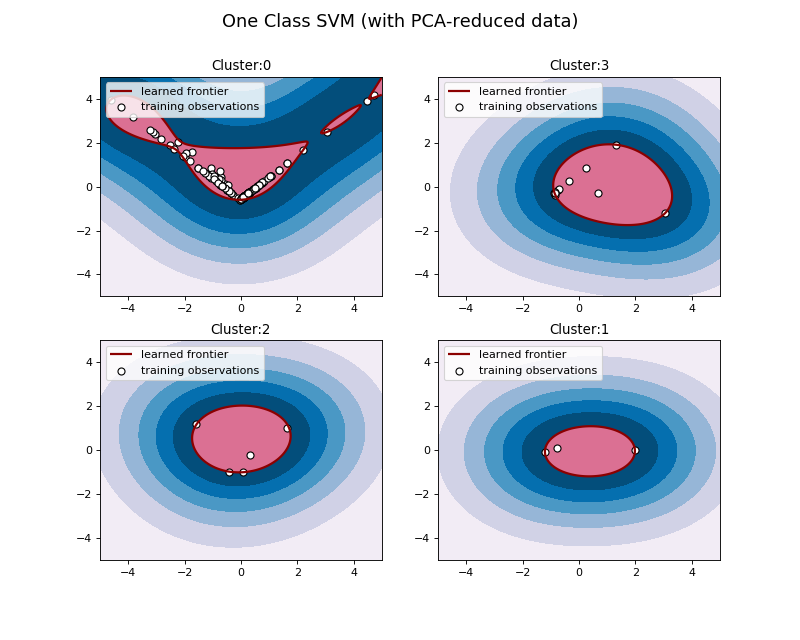
\includegraphics[width=0.80\textwidth]{one-class-SVM.png}
\caption{One Class SVM} \label{fig:one-class-SVM-in-program}
\end{figure}

\begin{minted}{Python}
def one_class_svm(feature_vector, cluster):
    X_train = feature_vector
    #Get scaler
    scaler = preprocessing.StandardScaler().fit(X_train)
    #Transform Traning data
    X_trans = scaler.transform(X_train)
    # fit the model
    clf = svm.OneClassSVM(nu=0.01, kernel="rbf", gamma=0.1)
    clf.fit(X_trans)
    clf.name = 'svm'
    return clf, scaler
\end{minted}
\textbf{Run One Class SVM}
\begin{minted}{Python}
clf_dict = dict()
scaler_dict = dict()
for cluster, df in cluster_feature_dict.items():
    clf_dict[cluster], scaler_dict[cluster] = one_class_svm(df, cluster)
\end{minted}
\pagebreak
\textbf{\Large{Clustering the data captured during attack}}
\begin{minted}{Python}
attack_sample_dir_name = 'attack_samp'
attack_sample_path = os.path.join(base_path, attack_sample_dir_name)
attack_sample_train_path = os.path.join(base_path, attack_sample_dir_name+'_train')
os.makedirs(attack_sample_train_path, exist_ok=True)
attack_cluster_path = os.path.join(attack_sample_train_path, 'cluster')
os.makedirs(attack_cluster_path, exist_ok=True)

files = sorted(glob.glob(os.path.join(attack_sample_path,'*')),  key=os.path.getmtime)
merge_count = np.genfromtxt(os.path.join(base_path,'merge_count'))

#Get centroids and feature list
centroids, features = read_centroid_features(centroid_filename, features_filename)

attack_dfs = merge_files(files, merge_count, features)

#Cluster all the samples and store them
centroids, features = read_centroid_features(centroid_filename, features_filename)
for i, attack_df in enumerate(attack_dfs):
    clustered_df = kmeans_clustering(attack_df, centroids)
    clustered_df.to_csv(os.path.join(attack_cluster_path,str(i+1)))

#Read clustered attack file
files = sorted(glob.glob(os.path.join(attack_cluster_path,'*')),  key=os.path.getmtime)
df = pd.read_csv(files[0], index_col=0)

train_tag_filename = 'ip_cluster_tag_train'
train_tag_file = os.path.join(base_path,train_tag_filename)
train_df = pd.read_csv(train_tag_file, index_col=0)
\end{minted}
\textbf{\Large{Detection}}
\begin{minted}{Python}
bad_ip_df = pd.DataFrame(columns=['ip', 'packet_count', 'percent_increase', 'cluster'])
for ip, row in df.iterrows():
    feature_row = row[:-1]
    cluster_value = row[-1]
    #cluster test
    if ip in train_df.index:
        packet_count = feature_row.sum()
        train_cluster = train_df.loc[ip]['cluster']
        #Train packet count
        train_packet_count = train_df.loc[ip]['packet_count']
        #Check how many percent increase in the average packet count
        percent_increase = ((packet_count - train_packet_count) / train_packet_count) * 100
        #Check the cluster value
        if(cluster_value == train_cluster):
            #SVM test: Check if its inside the boundary using one class svm
            X_test_tran = scaler_dict[cluster_value].transform([feature_row.values])
            #Check if its inside the cluster boundry using classifier
            prediction = clf_dict[cluster_value].predict(X_test_tran)
            if prediction == - 1:
                s = pd.Series([ip, packet_count, percent_increase, cluster_value], index=bad_ip_df.columns)
                bad_ip_df = bad_ip_df.append(s, ignore_index=True)
        else:
            s = pd.Series([ip, packet_count, percent_increase, cluster_value], index=bad_ip_df.columns)
            bad_ip_df = bad_ip_df.append(s, ignore_index=True)

bad_ip_df = bad_ip_df.set_index('ip')
print(bad_ip_df)
\end{minted}
\textbf{\Large{}}
\begin{minted}{Python}

\end{minted}
\end{document}
